\section{The Shape of a Can}
\label{sec:shape_of_a_can}	

\subsection*{Recommended Tutorials:}
\begin{itemize}[noitemsep]
	\item \nameref{chp:equation_solvers}, pg. \pageref{chp:equation_solvers}
	\item \nameref{chp:derivative}, pg. \pageref{chp:derivative}
\end{itemize}

\subsection*{Introduction:}
Your goal in this question is to design the most economical shape of a perfectly cylindrical can. 
\begin{figure}[h]
\centering
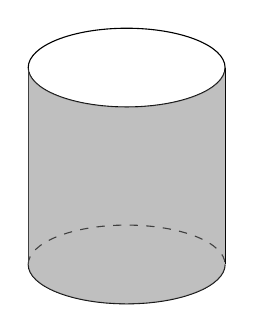
\begin{tikzpicture}
\draw (0,0) ellipse (1.25 and 0.5);
\draw (-1.25,0) -- (-1.25,-2.5);
\draw (-1.25,-2.5) arc (180:360:1.25 and 0.5);
\draw [dashed] (-1.25,-2.5) arc (180:360:1.25 and -0.5);
\draw (1.25,-2.5) -- (1.25,0);  
\fill [gray,opacity=0.5] (-1.25,0) -- (-1.25,-2.5) arc (180:360:1.25 and 0.5) -- (1.25,0) arc (0:180:1.25 and -0.5);
\end{tikzpicture}
\caption{A simple can in the shape of a circular cylinder.}
\end{figure}

First, let us assume the can has to hold a volume of 250 mL (250~cm$^3$). The cylindrical sides as well as the top and bottom circles are cut from sheets of aluminum. The material for the cylindrical sides of the cans is made from rectangles that are bent, so no material is wasted. However, some amount of material is always wasted when trying to cut circles from a sheet of metal. To make the most economical can, your goal is to reduce the \textit{total} amount of material needed, including any wasted metal.
%	\begin{center}
%	\psset{unit=0.8cm}
%    \begin{pspicture}(-1.5,-3)(1.5,1)
%    \psellipse(0,0)(1.5,0.7)
%    \psline(0,0)(1.5,0)
%    \psline(-1.5,0)(-1.5,-2)
%    \psline(1.5,0)(1.5,-2)
%    \psellipse(0,-2)(1.5,0.7)
%    \psframe*[linecolor=white](-1.47,-2)(1.47,-1)
%    \uput[u](0.75,-0.1){$r$}
%    \uput[d](1.8,-.8){$h$}
%    \end{pspicture}
%    \end{center}
%   	\caption{The can}
%   	\label{fig:can}
\begin{figure}[h]
\centering
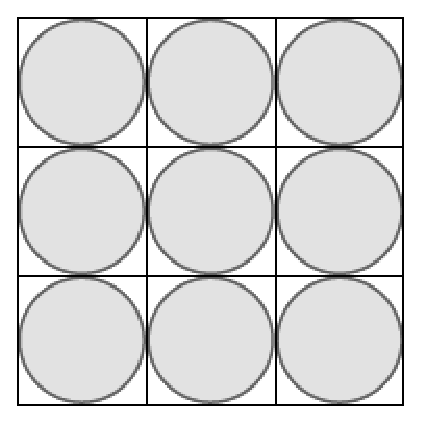
\includegraphics[scale=0.5]{activities/math112/figures/squares.eps}
\label{fig:square}
\caption{Cutting circles in a square pattern.}
\end{figure}
\begin{figure}[h]
\centering
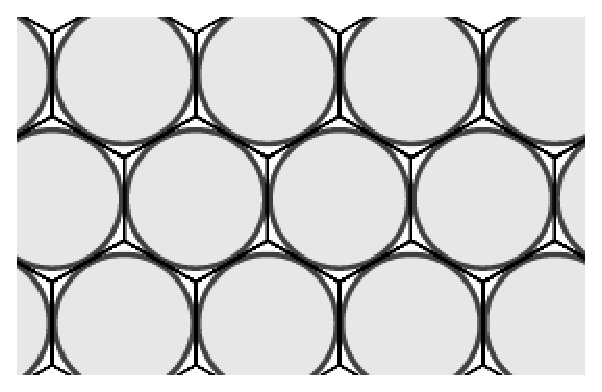
\includegraphics[scale=0.5]{activities/math112/figures/hexagons.eps}
\caption{Cutting circles in a hexagonal pattern.}
\label{fig:hexagon}
\end{figure}
    
If the circles are cut according to Figure \ref{fig:square}, then the total amount of material required for each can is a rectangle and two squares, which wastes a lot of material. If we plan to minimize the amount of material required, we will instead cut out circles according to Figure \ref{fig:hexagon}. The total area of material required for each can then becomes a rectangle and two hexagons.

\subsection*{Exercises:}
We will set up an equation for the total surface area of sheet metal required and then find when it is a minimum.
	\begin{enumerate}
	\marginnote[1cm]{Don't forget that the mathematical constant $\pi$ is represented in Maple as \texttt{Pi}.}\index{Pi}
	\item The side of the can is in the shape of a rectangle that has width $h$ and a length equal to the circumference of the lid. Give an equation for this area in terms of $r$ and $h$.
	\item The two hexagons that are needed for the top and bottom of the can circumscribe a circle of radius $r$. Give an equation for the area of this hexagon in terms of $r$. Figure \ref{hexagoncircle} may be helpful for splitting the hexagon up into six equilateral triangles.
\begin{figure}[h]
\caption{A hexagon circumscribing a circle.}
\centering
\begin{tikzpicture}
  \draw[] (0,0) circle (1.732050808cm);
  \node[regular polygon, regular polygon sides=6, draw, inner sep=1.2247cm] at (0,0) {};
  \draw (-1,1.732050808) -- (1,-1.732050808);
  \draw (-1,-1.732050808) -- (1,1.732050808);
  \draw (-2,0) -- (2,0);
  \draw (0,-1.732050808) -- (0,-1) node[right] {$r$} -- (0,0);
  \draw [<->] (-1,-2) -- (1,-2);
  \draw (0,-2) node [below] {$b$};
\end{tikzpicture}
%	\psset{unit=1cm}
%	\begin{pspicture}(-2,2)(2,-2)
%    \pspolygon(-1,1.732050808)(1,1.732050808)(2,0)(1,-1.732050808)(-1,-1.732050808)(-2,0)
%    \pscircle(0,0){1.732050808}
%    \psline(0,0)(-1,1.732050808)
%    \psline(0,0)(0,1.732050808)
%    \psline(0,0)(1,1.732050808)
%    \psline(0,0)(1.5,0.866025403)
%    \psline(0,0)(2,0)
%    \psline(0,0)(1.5,-0.866025403)
%    \psline(0,0)(1,-1.732050808)
%    \psline(0,0)(0,-1.732050808)
%    \psline(0,0)(-1,-1.732050808)
%    \psline(0,0)(-1.5,-0.866025403)
%    \psline(0,0)(-2,0)
%    \psline(0,0)(1.5,-0.866025403)
%    \psline(0,0)(-1.5,0.866025403)
%    \uput[60](0,0.866025403){$r$}
%    \end{pspicture}
\label{hexagoncircle}
\end{figure}
	\marginnote[-3cm]{Using trigonometric ratios of $\tfrac{\pi}{3}=60^\circ$ and $\tfrac{\pi}{6}=30^\circ$, it is possible to compute the length of $b$ in terms of $r$.}
	\marginnote[-1cm]{The area of each of the six triangles is $\tfrac{1}{2}br$.}
	\item Give an equation for the total area $A$ required (including waste) as a function of $r$ and $h$. This total area should include two hexagons and the rectangle that is used for the side of the can.
	\marginnote{The volume of a circular cylinder is \[ V=\pi r^2 h.\]}
	\item Given the required total volume $V=250$, use a substitution for $h$ to give the area from exercise 3 in terms of $r$ only. Assign this function as $A(r)$.
	\item Plot a graph of $A(r)$ over the interval $0 \leq r \leq 5$. Limit the vertical range to $-200 \leq A \leq  400$.
	\item Use the second derivative test to find the value of $r$ that minimizes the total area $A(r)$.
	\marginnote[-0.1cm]{For the second derivative test, find Type I critical numbers where $A'(r)=0$. Then show that $A''(r)>0$ for all $r>0$ to indicate that the area is an absolute minimum at this critical number.}
	\item Calculate the height of the can using this radius.
	\clearpage
	\marginnote{It can be shown that the ratio of height to radius of the optimized can is $\dfrac{h}{r} =~\dfrac{4\sqrt{3}}{\pi}$, regardless of volume.}
	\item Show that the ratio of height to radius is $\dfrac{h}{r} = \dfrac{4\sqrt{3}}{\pi} \approx 2.21$.
	\end{enumerate}
